\documentclass[14pt]{article}

\usepackage{graphics}
\usepackage{epsfig}
\usepackage{times}
\usepackage{amsmath}
\usepackage{subcaption}
\usepackage{multirow}
\usepackage{gensymb}
\usepackage{array}
\usepackage{float}
\usepackage{indentfirst}
\newcolumntype{P}[1]{>{\centering\arraybackslash}p{#1}}
\usepackage{booktabs, makecell}
\usepackage{diagbox}
\floatstyle{plaintop}
\restylefloat{table}
\usepackage{natbib}

\topmargin      0.0in
\headheight     0.0in
\headsep        0.0in
\oddsidemargin  0.0in
\evensidemargin 0.0in
\textheight     9.0in
\textwidth      6.5in

% additions to the course template
\usepackage{tabularx}
\usepackage{enumitem}
\usepackage{xcolor}
\usepackage{pgfgantt}
\usepackage[section]{placeins}
\usepackage[hidelinks]{hyperref}
\setlist{nosep}

\title{{\bf CENG391 Introduction to Image Understanding \\ Term Project Progress Report \\ 2026--2027 Fall Semester} \\
\it Project Title: DamageLens -- Disaster Damage Assessment from Pre/Post-Event Satellite Images \\
{\rm\normalsize Project \#30, Group G15}}

\date{November 2026}

\begin{document}

\pagestyle{plain}
\pagenumbering{roman}
\maketitle

\begin{figure}[H]
    \centering
    
\includegraphics[scale=0.35]{iyte_logo}
\end{figure}

\textbf{Group Members}
\begin{itemize}
    \item Yunus Melih Bozcan, 310201025
    \item \.{I}brahim \c{S}erkara, 310201115
    \item Canberk Y{\i}lmaz, 300201027
    \item Bora Toker, 310206004
\end{itemize}

\cleardoublepage
\pagenumbering{arabic}

\begin{abstract}
We are building a system that takes a pre-event and a post-event very-high-resolution satellite image of the same area, aligns them, finds damaged structures and summarises the damage on a map. The main case is the 6~February~2023 Kahramanmara\c{s} earthquakes. So far we have implemented data loaders for KATE-CD, xBD and raw Maxar Open Data imagery, two registration methods, classical change-detection baselines, a 6-channel U-Net and a grid-based spatial summary. On the KATE-CD test split the classical baselines reach F1 0.08--0.09, while the U-Net reaches 0.55, and 0.58 with misregistration augmentation. The main open problem is a domain gap: the same model flags almost no damage on raw Maxar scenes of a heavily damaged city centre. We have started hand-labelling raw tiles (18 of 64 processed) to fine-tune and evaluate on raw scenes.
\end{abstract}

\section{Introduction}
After a large earthquake, responders need to know quickly where buildings are damaged. Very-high-resolution satellite images taken before and after the event cover whole cities, but inspecting them by hand is slow. Automating this is an image understanding problem that combines image registration, change detection and semantic segmentation, and it has to cope with differences in season, illumination and viewing angle that are not damage.

Given co-located pre- and post-disaster images, the aim is to (i) align the pair, (ii) identify changed regions, (iii) segment damaged buildings and areas, (iv) summarise damage spatially, and (v) compare simple image-difference and feature baselines with a learned change-detection model. Our objectives are:
\begin{enumerate}
    \item a reproducible pipeline from raw imagery to a damage map (Python package \texttt{damagelens});
    \item a fair comparison of classical and learned change detection on the same test split;
    \item a measurement of how well a model trained on a curated dataset transfers to raw scenes.
\end{enumerate}

\section{Related Work}
\textbf{Classical change detection} compares the two images directly, through pixel or feature differences. A threshold can be selected from the histogram \citep{otsu1979}, structural similarity can replace the raw difference \citep{wang2004ssim}, and \citet{celik2009pca} cluster PCA features of difference blocks with $k$-means. These methods need no labels, but they react to every appearance change.

\textbf{Learned change detection} trains a segmentation network on labelled pairs. U-Net \citep{ronneberger2015unet} is a common backbone. \citet{daudt2018siamese} compare early fusion of the two images with Siamese fully convolutional networks, and \citet{chen2022bit} model the bitemporal context with a transformer. We start from an early-fusion U-Net because it is small and easy to train, and plan to compare it with a Siamese variant.

\textbf{Disaster datasets.} xBD \citep{gupta2019xbd} provides building polygons with four damage levels across many disaster types. BRIGHT \citep{chen2025bright} pairs optical pre-event with SAR post-event images. KATE-CD \citep{musaoglu2025kate} is a binary change-detection dataset from the 2023 Kahramanmara\c{s} earthquake. Our work differs in testing whether results on such curated data still hold on raw scenes of the affected cities.

\section{Dataset and Problem Definition}
The core task is binary segmentation of damaged pixels from a pre/post pair; a secondary task is 5-class segmentation (background and four damage levels). Table~\ref{tab:data} lists the data we use.

\begin{table}[H]
\centering\small
\caption{Data sources.}\label{tab:data}
\begin{tabularx}{\linewidth}{@{}lXll@{}}
\toprule
Dataset & Content & Labels & Role\\
\midrule
KATE-CD & 486 pre/post pairs, $512{\times}512$, 0.3--0.5\,m, Maxar and Pl\'eiades; split 404 / 44 / 38 & binary mask & main train/test\\
xBD & about 11k pairs, 19 disasters, Maxar & 4 damage levels & multi-class, transfer\\
Maxar Open Data & raw scenes of Kahramanmara\c{s} and Antakya, found through the STAC catalogue & ours (ongoing) & alignment, domain gap\\
\bottomrule
\end{tabularx}
\end{table}

We did not use UAV datasets with post-event images only (no pre image to align), BRIGHT (SAR post image, while our pipeline is optical), or construction and land-cover change datasets (not damage).

\textbf{Preprocessing.} KATE-CD masks are binarised. The two RGB images are stacked into a 6-channel input and normalised with ImageNet statistics. Augmentation uses flips and $90^\circ$ rotations, an optional random shift of the pre image (up to $\pm16$\,px) to simulate misregistration, and optionally 200 synthetic undamaged negatives (a pre image paired with a brightness- and colour-jittered copy of itself), because every KATE-CD tile contains damage. xBD polygons are rasterised to 5-class masks and downsampled $2\times$, with a deterministic train/test split. Raw Maxar windows are cut into $512{\times}512$ tiles.

\textbf{Hand labels.} We built a local web tool that shows pre and post tiles side by side for polygon annotation (damaged, destroyed, intact). For the Antakya centre area, 17 of 64 tiles are labelled and 1 is marked unusable, giving 312 building polygons (202 intact, 61 damaged, 49 destroyed). These labels are under review and are not yet used for training.

\section{Methodology}
The pipeline is: image pair $\rightarrow$ registration $\rightarrow$ change detection (baseline or U-Net) $\rightarrow$ damage mask $\rightarrow$ per-cell spatial summary.

\textbf{Registration.} (a) Phase correlation with sub-pixel upsampling \citep{guizar2008} estimates one translation per tile; shifts above 40\,px are rejected. (b) As a feature-based alternative, ORB keypoints \citep{rublee2011orb} with a RANSAC \citep{fischler1981ransac} affine fit.

\textbf{Classical baselines.} Image difference in Lab space after histogram matching, change vector analysis (CVA), CVA with Otsu thresholding, $1-$SSIM, and PCA with $k$-means on difference blocks. For non-building hazards we also implemented spectral indices (dNBR, $\Delta$NDVI, NDWI).

\textbf{Learned model.} A U-Net with a ResNet-18 encoder \citep{he2015resnet} pretrained on ImageNet, with 6 input channels (early fusion). The loss is binary cross-entropy (positive weight 5) plus Dice. We train for 30 epochs with batch size 8, AdamW (learning rate $3\cdot10^{-4}$, weight decay $10^{-4}$) and a cosine schedule. The best epoch and the decision threshold are chosen on the validation split, never on test. A 5-class variant is trained on xBD.

\textbf{Spatial summary.} Each tile of a raw scene is registered and predicted, and the damaged-pixel fraction of every 48\,m grid cell is drawn as a heat map.

\textbf{Implementation done so far.} Loaders for all three sources, both registration methods, the baselines, training and evaluation commands, the spatial-summary demo, the labelling tool, unit tests and continuous integration.

\section{Experiments and Results}
All results in this section are preliminary and come from single training runs. We report pixel-level F1 and IoU on the KATE-CD test split (38 tiles), and the xView2 score ($0.3\,F1_{\mathrm{loc}} + 0.7\,F1_{\mathrm{damage}}$) for xBD.

\begin{table}[H]
\centering\small
\caption{KATE-CD test split, pixel level.}\label{tab:kate}
\begin{tabular}{@{}lcc@{}}
\toprule
Method & F1 & IoU\\
\midrule
Image difference (Lab + histogram matching) & 0.083 & 0.043\\
CVA / $1-$SSIM / PCA-$k$-means / CVA+Otsu & 0.083--0.094 & 0.043--0.050\\
U-Net 5-class trained on xBD, applied directly (resolution matched) & 0.139 & 0.075\\
U-Net, xBD pretraining + KATE-CD fine-tuning & 0.500 & 0.333\\
U-Net, KATE-CD only & 0.552 & 0.382\\
\textbf{U-Net, KATE-CD + $\pm$16\,px shift + 200 negatives} & \textbf{0.579} & \textbf{0.407}\\
\bottomrule
\end{tabular}
\end{table}

\begin{table}[H]
\centering\small
\caption{Robustness to misregistration: pre image shifted synthetically, no registration (F1).}\label{tab:shift}
\begin{tabular}{@{}lcccc@{}}
\toprule
Shift (px) & 0 & 8 & 16 & 32\\
\midrule
U-Net, KATE-CD only & 0.552 & 0.468 & 0.365 & 0.328\\
U-Net, shift + negatives & 0.579 & 0.582 & 0.554 & 0.488\\
\bottomrule
\end{tabular}
\end{table}

On xBD the 5-class model reaches an xView2 score of 0.60. Figure~\ref{fig:pred} shows predictions, Figure~\ref{fig:base} the baselines and the effect of misalignment, and Figure~\ref{fig:map} the spatial summary on a raw scene.

\begin{figure}[H]
\centering
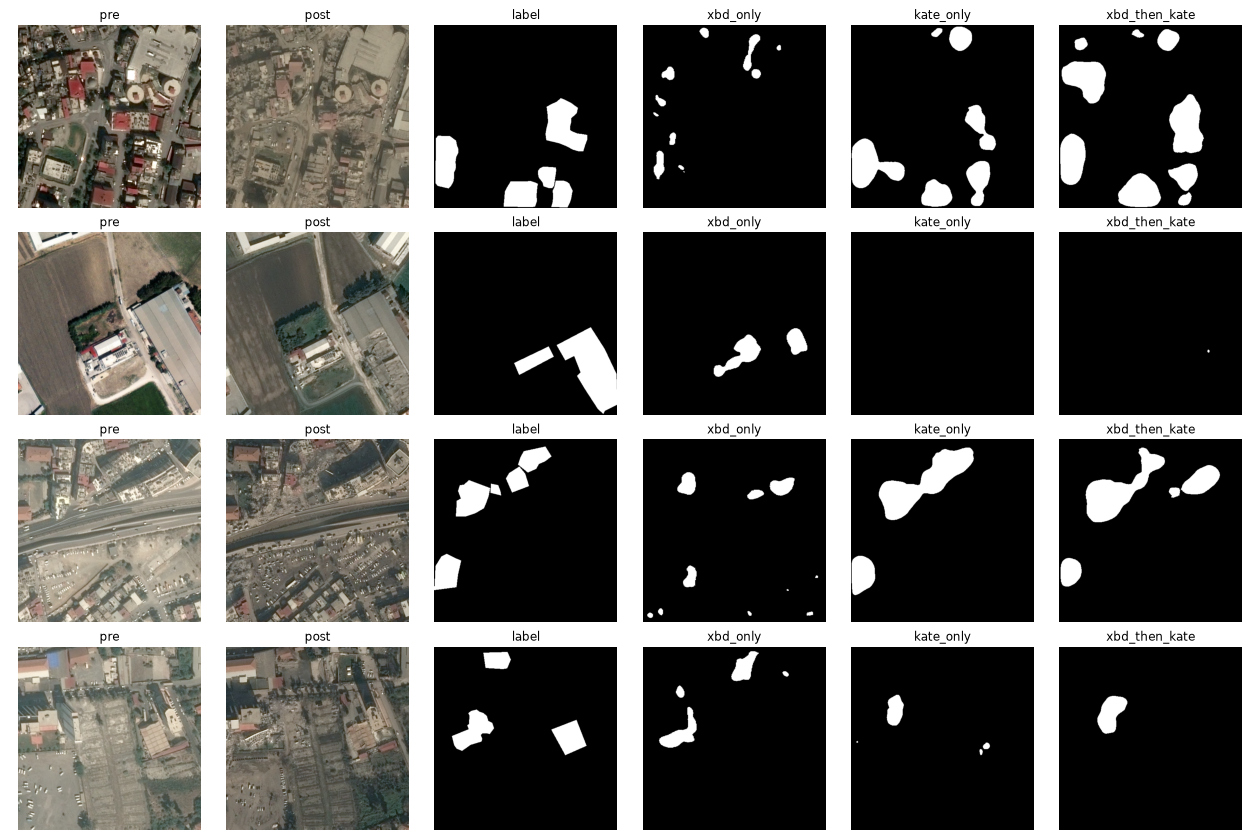
\includegraphics[width=\linewidth,height=0.42\textheight,keepaspectratio]{kate_predictions}
\caption{KATE-CD test tiles: pre, post, ground truth, and U-Net predictions of the xBD-only, KATE-CD-only and xBD-then-KATE-CD models.}\label{fig:pred}
\end{figure}

\begin{figure}[H]
\centering
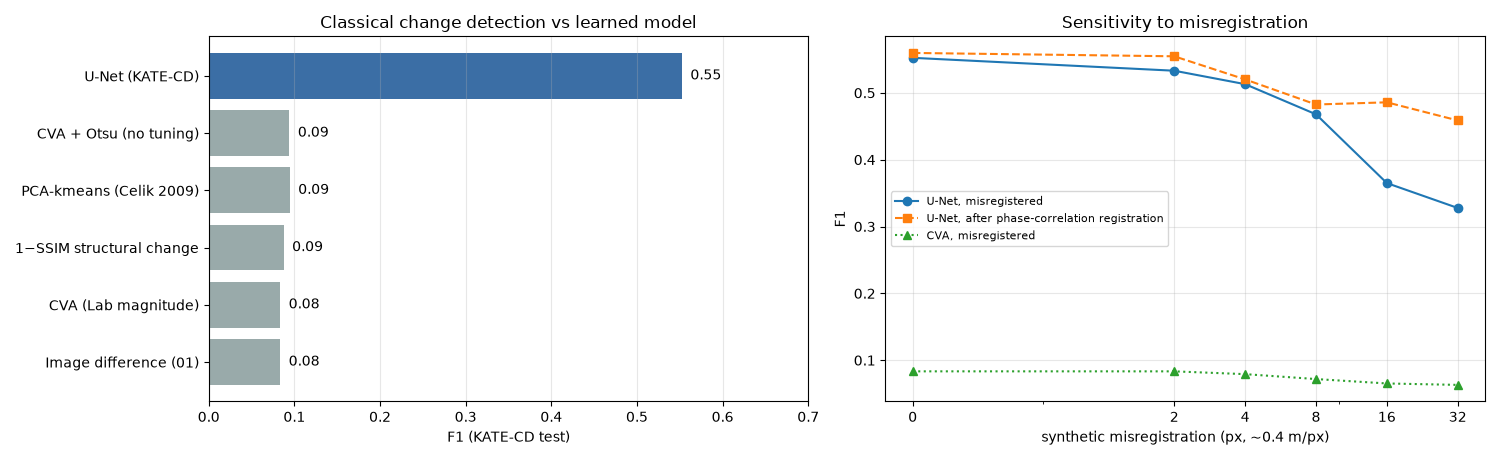
\includegraphics[width=\linewidth,height=0.42\textheight,keepaspectratio]{baselines_alignment}
\caption{Classical baselines and the effect of misregistration.}\label{fig:base}
\end{figure}

\begin{figure}[H]
\centering
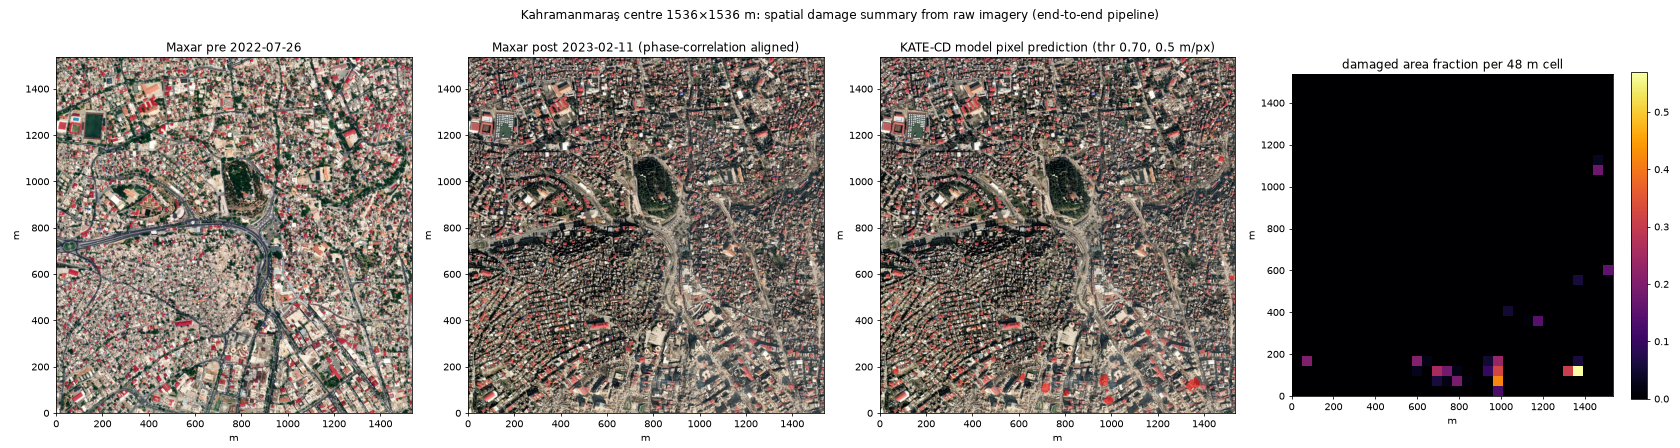
\includegraphics[width=\linewidth,height=0.42\textheight,keepaspectratio]{spatial_summary_kahramanmaras}
\caption{Spatial summary on raw Maxar imagery, Kahramanmara\c{s} centre (1.5\,km$^2$, 48\,m cells).}\label{fig:map}
\end{figure}

\section{Discussion}
The learned model reaches about six times the F1 of the classical baselines (Table~\ref{tab:kate}). The baselines respond to all appearance change (season, shadow, snow), not only to damage. A 16\,px misalignment lowers F1 from 0.55 to 0.36; phase correlation recovers it to 0.49, and training with random shifts makes the model almost insensitive up to 16\,px (Table~\ref{tab:shift}). Raw Maxar pairs of Kahramanmara\c{s} are misaligned by a median of 12--16\,px (about 6--8\,m), so this matters in practice. Knowledge from xBD did not transfer well to T\"urkiye (F1 0.14 without fine-tuning), and xBD pretraining did not help fine-tuning.

\subsection{Challenges}
\begin{itemize}
    \item \textbf{Domain gap (main problem).} Models with F1 0.55--0.58 on KATE-CD flag only 0.6\,\% of pixels as damaged in the heavily damaged Kahramanmara\c{s} centre on raw Maxar imagery (0.09\,\% for the shift + negatives model), and under 1\,\% even at threshold 0.3. Threshold and alignment do not explain this; scene selection, season and processing differ.
    \item \textbf{No undamaged tiles in KATE-CD,} so the false-alarm rate cannot be measured; synthetic negatives are only a stand-in.
    \item \textbf{No georeferenced ground truth for T\"urkiye.} KATE-CD as released has no coordinates, the HOT OSM export was empty, and Copernicus EMS EMSR648 access still has to be checked.
    \item \textbf{Season, snow, cloud and parallax} create false changes, and one translation per tile cannot correct tall buildings.
    \item \textbf{Small test set} (38 tiles): final results should be mean $\pm$ standard deviation over 3 seeds or $k$-fold.
    \item \textbf{Evaluation leakage, found and fixed:} the first xBD split depended on Python's hash seed, so test overlapped with training (xView2 0.62 instead of 0.60). The split is now deterministic.
\end{itemize}

\section{Conclusion and Future Work}
An end-to-end pipeline runs on open data, and the learned model clearly outperforms the classical baselines on KATE-CD. It does not yet work reliably on raw scenes, so the project objectives are only partly achieved.

\subsection{Next Steps}
\begin{enumerate}
    \item Finish hand-labelling raw Maxar tiles, then fine-tune and evaluate on raw scenes.
    \item Compare a Siamese, feature-difference model with the early-fusion U-Net.
    \item Add real undamaged negatives, a snow/cloud mask and colour/shadow augmentation; evaluate over multiple seeds.
    \item Compare ORB + RANSAC with phase correlation on real pairs.
    \item Build a district-level summary and map interface, then write the final report and presentation.
\end{enumerate}

\section{Gantt Chart and Task Assignments}
Owners: MB = Yunus Melih Bozcan, \.{I}\c{S} = \.{I}brahim \c{S}erkara, CY = Canberk Y{\i}lmaz, BT = Bora Toker. The dark part of a bar is the completed share; the red line marks the report date (27 November 2026). Table~\ref{tab:status} gives exact dates and percentages.

\begin{center}
\begin{ganttchart}[
 time slot format=isodate, x unit=0.08cm, y unit chart=0.46cm, y unit title=0.5cm,
 vgrid={*6{draw=none},dotted}, today=2026-11-27, today rule/.style={draw=red, thick}, today label={},
 bar/.append style={fill=teal!60, draw=gray!60}, bar incomplete/.append style={fill=gray!25},
 bar height=0.6, progress label text={}, bar label font=\scriptsize, group label font=\scriptsize\bfseries,
 group/.append style={fill=black!70}, group peaks height=0.15, title label font=\scriptsize
]{2026-09-21}{2027-01-17}
 \gantttitlecalendar{month=shortname} \\
 \ganttgroup{Phase 1: feasibility and exploration}{2026-09-28}{2026-11-27} \\
 \ganttbar[progress=100]{Literature and similar-project review [MB, \.{I}\c{S}, CY, BT]}{2026-09-28}{2026-10-25} \\
 \ganttbar[progress=100]{Dataset discovery and access (KATE-CD, xBD, Maxar) [\.{I}\c{S}, MB]}{2026-10-05}{2026-11-08} \\
 \ganttbar[progress=100]{Data loaders and preprocessing [MB]}{2026-10-12}{2026-10-31} \\
 \ganttbar[progress=100]{Registration (phase corr., ORB) [MB]}{2026-10-19}{2026-11-08} \\
 \ganttbar[progress=100]{Classical baselines [MB]}{2026-10-26}{2026-11-13} \\
 \ganttbar[progress=100]{U-Net, shift augmentation, negatives [MB]}{2026-11-02}{2026-11-22} \\
 \ganttbar[progress=100]{xBD 5-class and other hazards [MB]}{2026-11-09}{2026-11-22} \\
 \ganttbar[progress=100]{Spatial summary demo [MB]}{2026-11-16}{2026-11-25} \\
 \ganttbar[progress=100]{Labelling tool, tests, CI [MB]}{2026-11-16}{2026-11-27} \\
 \ganttbar[progress=90]{Progress report [CY, MB]}{2026-11-16}{2026-11-27} \\
 \ganttgroup{Phase 2: raw-scene adaptation}{2026-11-20}{2027-01-03} \\
 \ganttbar[progress=28]{Hand-label raw Maxar tiles [BT, CY]}{2026-11-20}{2026-12-11} \\
 \ganttbar[progress=10]{KATE-CD licence and coordinates [\.{I}\c{S}]}{2026-11-23}{2026-12-11} \\
 \ganttbar[progress=0]{ORB vs phase correlation on Maxar [\.{I}\c{S}]}{2026-11-30}{2026-12-11} \\
 \ganttbar[progress=0]{Siamese model vs U-Net [MB]}{2026-11-30}{2026-12-18} \\
 \ganttbar[progress=0]{Real negatives, snow/cloud mask [\.{I}\c{S}]}{2026-12-07}{2026-12-20} \\
 \ganttbar[progress=0]{Colour and shadow augmentation [BT]}{2026-12-07}{2026-12-20} \\
 \ganttbar[progress=0]{Fine-tune and evaluate on raw scenes [MB, BT]}{2026-12-14}{2026-12-31} \\
 \ganttbar[progress=0]{District summary and map UI [CY, \.{I}\c{S}]}{2026-12-14}{2027-01-03} \\
 \ganttbar[progress=0]{Multi-seed / k-fold evaluation [CY]}{2026-12-21}{2027-01-03} \\
 \ganttgroup{Phase 3: delivery}{2027-01-01}{2027-01-15} \\
 \ganttbar[progress=0]{Final report [MB, \.{I}\c{S}, CY, BT]}{2027-01-01}{2027-01-12} \\
 \ganttbar[progress=0]{Presentation [MB, \.{I}\c{S}, CY, BT]}{2027-01-06}{2027-01-15}
\end{ganttchart}
\end{center}

\begin{table}[H]
\centering\scriptsize
\caption{Task assignments and status.}\label{tab:status}
\begin{tabularx}{\linewidth}{@{}Xlllr@{}}
\toprule
Task & Owner(s) & Start -- End & Status & Done\\
\midrule
Literature and similar-project review & Bozcan, \c{S}erkara, Y{\i}lmaz, Toker & 09-28 -- 10-25 & completed & 100\%\\
Dataset discovery and access (KATE-CD, xBD, Maxar) & \c{S}erkara, Bozcan & 10-05 -- 11-08 & completed & 100\%\\
Data loaders and preprocessing & Bozcan & 10-12 -- 10-31 & completed & 100\%\\
Registration (phase corr., ORB) & Bozcan & 10-19 -- 11-08 & completed & 100\%\\
Classical baselines & Bozcan & 10-26 -- 11-13 & completed & 100\%\\
U-Net, shift augmentation, negatives & Bozcan & 11-02 -- 11-22 & completed & 100\%\\
xBD 5-class and other hazards & Bozcan & 11-09 -- 11-22 & completed & 100\%\\
Spatial summary demo & Bozcan & 11-16 -- 11-25 & completed & 100\%\\
Labelling tool, tests, CI & Bozcan & 11-16 -- 11-27 & completed & 100\%\\
Progress report & Y{\i}lmaz, Bozcan & 11-16 -- 11-27 & ongoing & 90\%\\
Hand-label raw Maxar tiles & Toker, Y{\i}lmaz & 11-20 -- 12-11 & ongoing & 28\%\\
KATE-CD licence and coordinates & \c{S}erkara & 11-23 -- 12-11 & ongoing & 10\%\\
ORB vs phase correlation on Maxar & \c{S}erkara & 11-30 -- 12-11 & upcoming & 0\%\\
Siamese model vs U-Net & Bozcan & 11-30 -- 12-18 & upcoming & 0\%\\
Real negatives, snow/cloud mask & \c{S}erkara & 12-07 -- 12-20 & upcoming & 0\%\\
Colour and shadow augmentation & Toker & 12-07 -- 12-20 & upcoming & 0\%\\
Fine-tune and evaluate on raw scenes & Bozcan, Toker & 12-14 -- 12-31 & upcoming & 0\%\\
District summary and map UI & Y{\i}lmaz, \c{S}erkara & 12-14 -- 01-03 & upcoming & 0\%\\
Multi-seed / k-fold evaluation & Y{\i}lmaz & 12-21 -- 01-03 & upcoming & 0\%\\
Final report & Bozcan, \c{S}erkara, Y{\i}lmaz, Toker & 01-01 -- 01-12 & upcoming & 0\%\\
Presentation & Bozcan, \c{S}erkara, Y{\i}lmaz, Toker & 01-06 -- 01-15 & upcoming & 0\%\\
\bottomrule
\end{tabularx}
\end{table}

\section{Team Contributions}
\begin{description}
    \item[Yunus Melih Bozcan:] repository and pipeline: data loaders, registration, baselines, U-Net training and evaluation, spatial summary, labelling tool, tests and CI.
    \item[\.{I}brahim \c{S}erkara:] survey of pre/post satellite datasets and their access routes, used to select the data in Table~\ref{tab:data}; contacted ITÜ CSCRS about the KATE-CD licence.
    \item[Canberk Y{\i}lmaz:] similar-project review; prepared this progress report: wrote the draft, checked it against the course template and requirements, and built the Gantt chart and task table with the group.
    \item[Bora Toker:] initial research notes on methods and datasets; hand-labelling of Antakya tiles (17 labelled, 1 skipped).
\end{description}

\section*{GenAI Usage Disclosure}
\begin{itemize}
    \item Claude Opus 5.5 (\texttt{claude-opus-5-5}), through Claude Code: drafted the first LaTeX version of this report from the repository README, code and results, and checked dataset links.
    \item Claude Sonnet 5.5 (\texttt{claude-sonnet-5-5}), through Claude Code: moved the draft into the course template, drafted the Related Work section and bibliography, and updated the task status. Numbers come from our own experiments and repository.
    \item Antigravity 2.34 with Gemini 4 Hydrogen: used by Bora Toker only to set up the repository locally; no code was changed with it.
\end{itemize}

\setlength{\bibsep}{2pt}
\bibliographystyle{chicago}
\bibliography{literature}

\end{document}
